\documentclass{standalone}
% \documentclass{article}

\usepackage{tikz}

\begin{document}

\begin{tikzpicture}

\node at (0, 0) {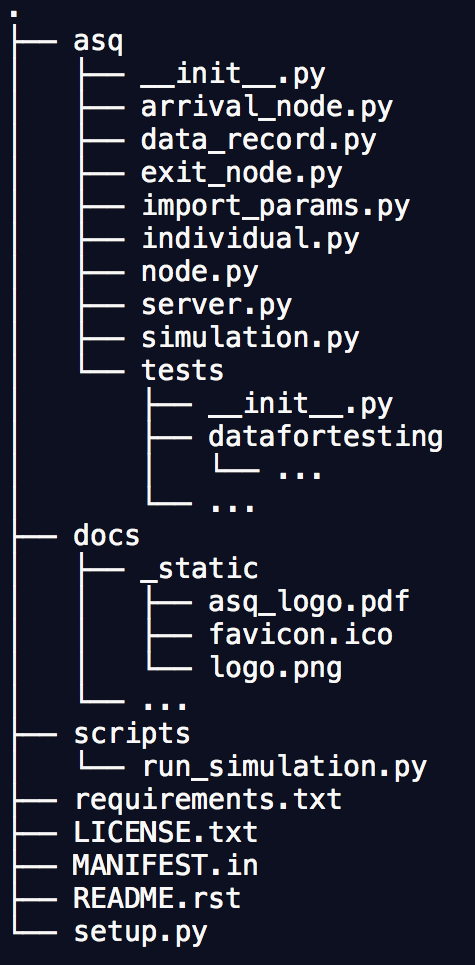
\includegraphics{repostructure}};

\draw[ultra thick,draw=magenta,fill=magenta,opacity=0.2] (-7, -8.2) rectangle (7.5, -10.6);

\draw[ultra thick,draw=blue,fill=blue,opacity=0.2] (-7, 4.5) rectangle (7.5, 16.5);

\draw[ultra thick,draw=red,fill=red,opacity=0.2] (-7, 4.5) rectangle (7.5, -1.3);

\draw[ultra thick,draw=green,fill=green,opacity=0.2] (-7, -10.6) rectangle (7.5, -16.5);

\pause

\draw[ultra thick,draw=yellow,fill=yellow,opacity=0.2] (-7, -1.3) rectangle (7.5, -8.2);


\end{tikzpicture}

\end{document}
